\documentclass[10pt, oneside]{amsart}
\pagestyle{plain}
\usepackage{parskip, graphicx, amssymb, amsmath, epstopdf, enumitem, amsthm, pgfplots, tikz, tcolorbox, caption, subcaption, multicol}
\pgfplotsset{compat=1.18}
\DeclareGraphicsRule{.tif}{png}{.png}{`convert #1 `dirname #1`/`basename #1 .tif`.png}
\usetikzlibrary{shapes.geometric}

    
\newtheorem{thm}{Theorem}

\setlength{\tabcolsep}{20pt}
\renewcommand{\arraystretch}{1.5}

\textheight 642pt
\footskip 35pt
\voffset = -40pt
\addtolength{\oddsidemargin}{-.25in}
\addtolength{\textwidth}{0.5in}

\begin{document}
{\bf Math 1271 - Worksheet 2} \hfill \emph{9/10/2026}

{\bf\Large 1.2 - Intro to Limits}

\medskip

\begin{enumerate}[leftmargin=0pt]

\item[1.] The graph\footnote{Source: Salas, Etgen, Hille - \emph{Calculus} (10th Ed)}
 of a function $f(x)$ is given below. Use the graph to evaluate the following, if possible. If a value does not exist, write ``DNE" and explain why the value does not exist.

\begin{center}
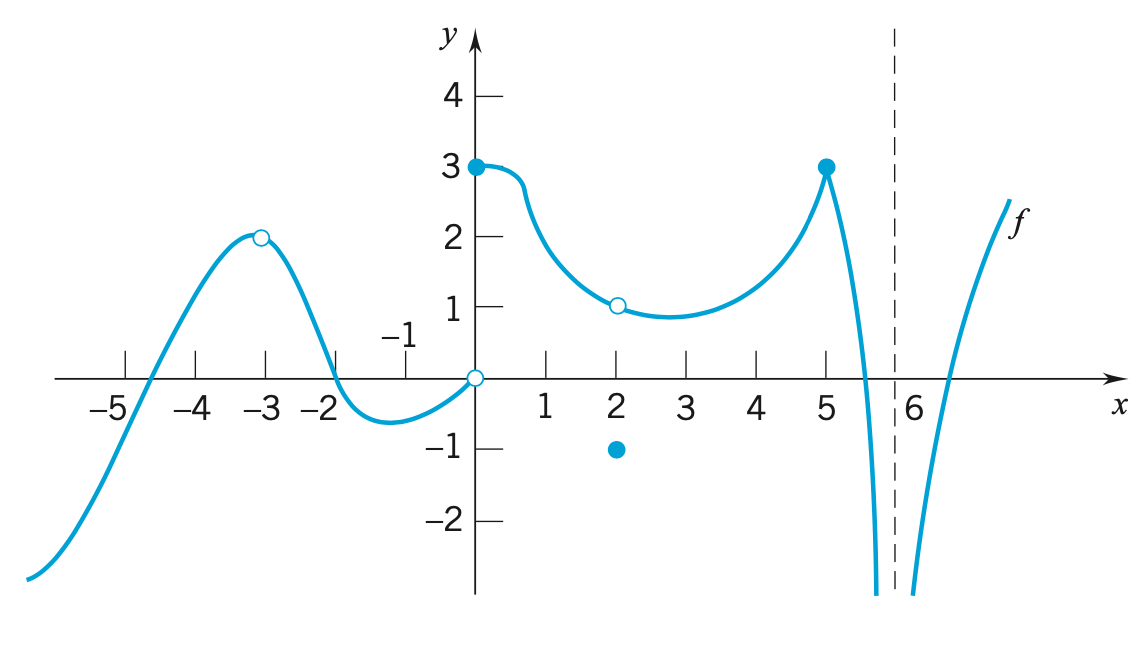
\includegraphics[scale=0.53]{wkst3img.png}
\end{center}

\medskip

\begin{multicols}{2}

\begin{enumerate}

\item[(a)] $f(-3)$

\vspace{0.83in}

\item[(b)] $f(0)$

\vspace{0.83in}

\item[(c)] $f(2)$

\vspace{0.8in}

\item[(d)] $f(5)$

\vspace{0.8in}

\item[(e)] $f(6)$

\vfill

\item[(f)] $\displaystyle\lim_{x\to -3} f(x)$

\vspace{0.75in}

\item[(g)] $\displaystyle\lim_{x\to 0} f(x)$

\vspace{0.75in}

\item[(h)] $\displaystyle\lim_{x\to 2} f(x)$

\vspace{0.75in}

\item[(i)] $\displaystyle\lim_{x\to 5} f(x)$

\vspace{0.75in}

\item[(j)] $\displaystyle\lim_{x\to 6} f(x)$

\vfill

\end{enumerate}
\end{multicols}

\newpage


\item[2.] Estimate the value of each of the following limits by constructing appropriate tables of values. Use a graphing tool (Desmos, etc.) to plot each function on an appropriate interval to check your result visually. 

\medskip

\begin{enumerate}

\item[(a)] $\displaystyle\lim_{x\to 1}\frac{x^2-1}{x-1}$

\vfill

\item[(b)] $\displaystyle\lim_{x\to 0}\frac{(2+x)^3-8}{x}$

\vfill

\item[(c)] $\displaystyle\lim_{x\to0}\frac{\sqrt{x+1}-1}{x}$

\vfill

\end{enumerate}
\item[1.] On the previous worksheet, you used a table of values to investigate each of the following limits. Use algebra to show that your answers are correct. (Please show all work!)

\medskip

\begin{enumerate}

\item[(a)] $\displaystyle\lim_{x\to 1}\frac{x^2-1}{x-1}$

\vfill

\item[(b)] $\displaystyle\lim_{x\to 0}\frac{(2+x)^3-8}{x}$

\vfill

\item[(c)] $\displaystyle\lim_{x\to0}\frac{\sqrt{x+1}-1}{x}$

\vfill

\end{enumerate}

\newpage


\item[2.] Two functions, $f(x)$ and $g(x)$, are graphed below:

\begin{multicols}{2}

\begin{enumerate}

\item[]

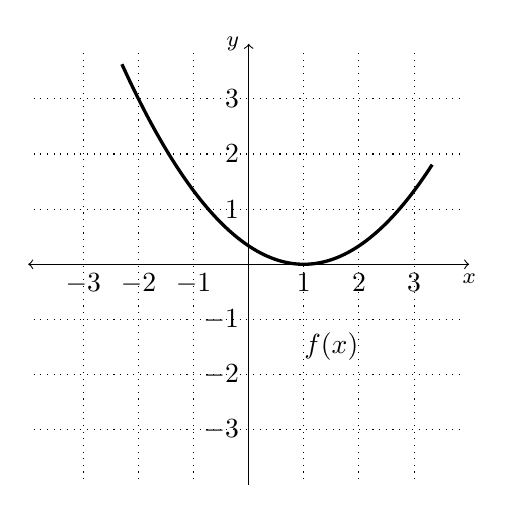
\begin{tikzpicture}[scale=0.7]
 Grid
\draw[dotted] (-3.9,-3.9) grid (3.9,3.9); 
 Axes
\draw[<->] (-4,0) -- (4,0)node[anchor=north] {\footnotesize{$x$}};
\draw[->] (0,-4)--(0,4)node[anchor=east] {\footnotesize{$y$}};

\draw[very thick,-] [smooth,samples=100,domain=-2.3:3.33] plot({\x},{(1/3)*((\x)-1)^2});

\node at (1.5,-1.5) {$f(x)$};

\node[anchor=north] at (-1,0)  {$-1$};
\node[anchor=north] at (-2,0)  {$-2$};
\node[anchor=north] at (-3,0)  {$-3$};
\node[anchor=north] at (1,0)  {$1$};
\node[anchor=north] at (2,0)  {$2$};
\node[anchor=north] at (3,0)  {$3$};

\node[anchor=east] at (0,-3)  {$-3$};
\node[anchor=east] at (0,-2)  {$-2$};
\node[anchor=east] at (0,-1)  {$-1$};
\node[anchor=east] at (0,1)  {$1$};
\node[anchor=east] at (0,2)  {$2$};
\node[anchor=east] at (0,3)  {$3$};
\end{tikzpicture}

\columnbreak

\item[]

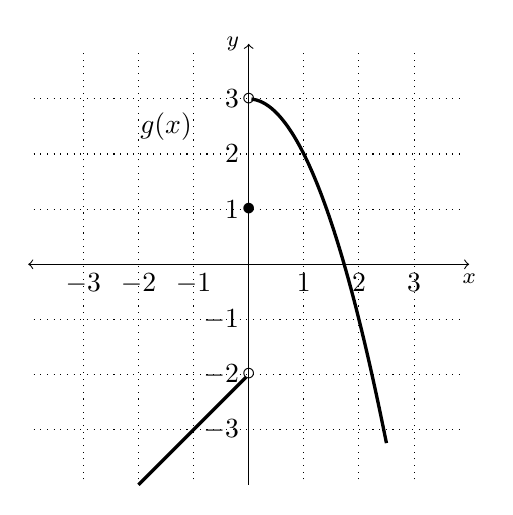
\begin{tikzpicture}[scale=0.7]
 Grid
\draw[dotted] (-3.9,-3.9) grid (3.9,3.9); 
 Axes
\draw[<->] (-4,0) -- (4,0)node[anchor=north] {\footnotesize{$x$}};
\draw[->] (0,-4)--(0,4)node[anchor=east] {\footnotesize{$y$}};

\draw[very thick,-] [smooth,samples=100,domain=-2:-0.05] plot({\x},{(\x)-2});

\node at (0,-2) {$\circ$};

\node at (0,1) {$\bullet$};

\node at (0,3) {$\circ$};

\node at (-1.5, 2.5) {$g(x)$};

\draw[very thick,-] [smooth,samples=100,domain=0.05:2.5] plot({\x},{3-(\x)^2});

\node[anchor=north] at (-1,0)  {$-1$};
\node[anchor=north] at (-2,0)  {$-2$};
\node[anchor=north] at (-3,0)  {$-3$};
\node[anchor=north] at (1,0)  {$1$};
\node[anchor=north] at (2,0)  {$2$};
\node[anchor=north] at (3,0)  {$3$};

\node[anchor=east] at (0,-3)  {$-3$};
\node[anchor=east] at (0,-2)  {$-2$};
\node[anchor=east] at (0,-1)  {$-1$};
\node[anchor=east] at (0,1)  {$1$};
\node[anchor=east] at (0,2)  {$2$};
\node[anchor=east] at (0,3)  {$3$};
\end{tikzpicture}

\end{enumerate}
\end{multicols}

(If necessary, you may assume that $f(0)=\frac{1}{3}$.)

Use these graphs (and limit laws) to evaluate each of the following limits. If a limit does not exist, then write ``DNE" and explain why the limit does not exist. 

\begin{enumerate}

\item[(a)] $\displaystyle\lim_{x\to 1} \dfrac{1}{2+f(x)}$

\vfill

\item[(b)] $\displaystyle\lim_{x\to 0}[f(x)+g(x)]$

\vfill

\item[(c)] $\displaystyle\lim_{x\to -1} f(x^2)$

\vfill

\item[(d)] $\displaystyle\lim_{x\to 1} g(f(x))$  (Hint: Be careful!)

\vfill

\end{enumerate}

\newpage


\item[3.] You may assume that the function $y=\dfrac{1-\cos(x)}{x^2}$ satisfies the inequalities
$$\frac{1}{2}-\frac{x^2}{24}<\frac{1-\cos(x)}{x^2}<\frac{1}{2}$$
for all values of $x$ close to $0$. (You can learn where this comes from in Calculus II!) Use this information as needed to find the exact values of each limit below (if a limit does not exist, write ``DNE"). If the Squeeze Theorem is used, show all work; if not, then explain why the theorem does not apply.

\begin{enumerate}

\item[(a)] $\displaystyle\lim_{x\to 0}\frac{1-\cos(x)}{x^2}$

\vfill

\item[(b)] $\displaystyle\lim_{x\to \pi}\frac{1-\cos(x)}{x^2}$

\vfill

\end{enumerate}


\end{enumerate}

\end{document}
